  \documentclass[final]{beamer} % beamer 3.10: do NOT use option hyperref={pdfpagelabels=false} !
  %\documentclass[final,hyperref={pdfpagelabels=false}]{beamer} % beamer 3.07: get rid of beamer warnings
  \mode<presentation> {  %% check http://www-i6.informatik.rwth-aachen.de/~dreuw/latexbeamerposter.php for examples
    \usetheme{I6pd2}    %% you should define your own theme e.g. for big headlines using your own logos 
  }
  \usepackage[english]{babel}
  \usepackage[latin1]{inputenc}
  \usepackage{amsmath,amsthm, amssymb, latexsym}
  \usepackage[absolute,overlay]{textpos}
  \usepackage{pbox}
  %\usepackage{times}\usefonttheme{professionalfonts}  % times is obsolete
  \usefonttheme[onlymath]{serif}
  \boldmath
  \usepackage[orientation=portrait,size=a0,scale=1.5,debug]{beamerposter}                       % e.g. for DIN-A0 poster
  %\usepackage[orientation=portrait,size=a1,scale=1.4,grid,debug]{beamerposter}                  % e.g. for DIN-A1 poster, with optional grid and debug output
  %\usepackage[size=custom,width=200,height=120,scale=2,debug]{beamerposter}                     % e.g. for custom size poster
  %\usepackage[orientation=portrait,size=a0,scale=1.0,printer=rwth-glossy-uv.df]{beamerposter}   % e.g. for DIN-A0 poster with rwth-glossy-uv printer check
  % ...
  %
  \title[Deep Learning for Feature Location]{Exploring the Use of Deep Learning for Feature Location}
  \author[Corley et al.]{Christopher S. Corley$^{1}$, Kostadin Damevski$^2$, Nicholas A. Kraft$^3$}
  \institute[]{$^1$University of Alabama \\
               $^2$Virginia Commonwealth University \\
               $^3$ABB Corporate Research}
  \date{}
 
  \begin{document}
  \begin{frame}


  \begin{columns}[t]
    % ---------------------------------------------------------%
    % Set up a column 
    \begin{column}{.49\textwidth}
      \begin{beamercolorbox}[center,wd=\textwidth]{postercolumn}
        \begin{minipage}[T]{.95\textwidth}  % tweaks the width, makes a new \textwidth


            \begin{block}{Key Ideas}
              \begin{itemize}
                \item 
                  Exploration of the use of a particular deep learning model, document vectors (DVs), for feature location of source code
                \item
                  DVs seem well suited to use with source code,
                  because they both capture the influence of context
                  on each term in a corpus and map terms into a
                  continuous semantic space that encodes semantic
                  relationships such as synonymy
               \item
                  Preliminary results indicate that a feature
                  location technique (FLT) based on DVs can outperform
                  an analogous FLT based on Latent Dirichlet
                  Allocation (LDA).
              \end{itemize}              
             \end{block}
 

            \vskip 1cm


            \begin{block}{Semantic Similarity Example for ArgoUML v0.22}
              
              \begin{table}[t]
                \centering
                \begin{tabular}{p{0.32\linewidth}p{0.63\linewidth}}
                  \hline
                      {\bf Example Term(s)} & {\bf Semantically Similar Terms and Weight}\\ 
                      \hline
                      save & (saved 0.69), (pcs 0.64), (exists 0.63), (projects 0.60), (close 0.61), (file 0.60) \\ \hline
                      file & (filter 0.78), (zip 0.74), (exists 0.74), (persister 0.71), (files 0.69), (directory 0.69) \\ \hline
                      file + save & (exists 0.77), (saved 0.74), (filter 0.73), (zip 0.72), (unable 0.67), (projects 0.67), (persister 0.67), (files 0.66), (cant 0.66), (scheme 0.65) \\ \hline
                      explorer + diagrams \newline - creating & (nodes 0.71), (deletion 0.67), (perspectives 0.65), (perspective 0.60), (updated 0.60), (modified 0.60)\\
                      \hline
                \end{tabular}
              \end{table}
            \end{block}
              
        \end{minipage}
      \end{beamercolorbox}
    \end{column}
    % ---------------------------------------------------------%
    % end the column

    % ---------------------------------------------------------%
    % Set up a column 
    \begin{column}{.49\textwidth}
      \begin{beamercolorbox}[center,wd=\textwidth]{postercolumn}
        \begin{minipage}[T]{.95\textwidth} % tweaks the width, makes a new \textwidth

          \begin{block}{Deep Neural Network for Source Code}

            \centering
            Figure: The neural network encodes each term and its context\\ 
            into a semantic vector representation.\par

            \vskip 0.5cm

            \begin{center}
              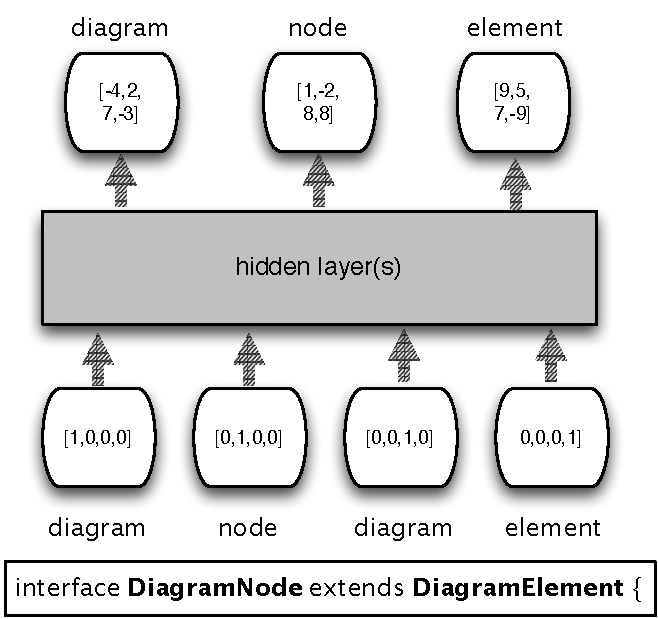
\includegraphics[width=.9\linewidth]{../figures/neuralnet.pdf}
            \end{center}
          \end{block}
          
          \vskip 1cm
          
          % ---------------------------------------------------------%
          % end the column
        \end{minipage}
      \end{beamercolorbox}
    \end{column}
    % ---------------------------------------------------------%
    % end the column

  \end{columns} 


  \vskip 1cm
    
  \begin{beamercolorbox}[center]{AAAA}
    \begin{minipage}[T]{.97\textwidth}  % tweaks the width, makes a new \textwidth
      \begin{block}{Experimental Results}

        \centering
        Figure: Mean Reciprocal Rank (MRR) computed on the the feature location dataset by Dit et al. [MSR'13]\par
        

        \hfill
        \begin{columns}
        \begin{column}{0.45\textwidth}
          \vspace{2.95cm}
          \begin{tabular}{llccccc}
            \hline
            {\bf System} & {\bf Approach} & {\bf 100} & {\bf 200} & {\bf 300} & {\bf 400} & {\bf 500}         \\
            \hline
            & LDA           & 0.0175       & 0.0295       & 0.0271       & {\bf 0.0611} & 0.0220       \\
            ArgoUML v0.22      & DV\ Inference & 0.0115       & 0.0105       & 0.0096       & 0.0184       & 0.0162       \\
            & DV\ Summation & {\bf 0.0775} & {\bf 0.0570} & {\bf 0.0625} & 0.0587       & {\bf 0.0601} \\
            \hline
            & LDA           & 0.0441       & 0.0373       & 0.0655       & {\bf 0.0779} & 0.0344       \\
            ArgoUML v0.24      & DV\ Inference & 0.0246       & 0.0152       & 0.0260       & 0.0258       & 0.0380       \\
            & DV\ Summation & {\bf 0.0827} & {\bf 0.0906} & {\bf 0.0874} & 0.0691       & {\bf 0.0942} \\
            \hline
            & LDA           & 0.0493       & 0.0628       & {\bf 0.0857} & 0.0703       & {\bf 0.0811} \\
            ArgoUML v0.26.2    & DV\ Inference & 0.0404       & 0.0218       & 0.0290       & 0.0364       & 0.0403       \\
            & DV\ Summation & {\bf 0.0847} & {\bf 0.0890} & 0.0813       & {\bf 0.0834} & 0.0805       \\
            \hline
            & LDA           & 0.0055       & 0.0364       & {\bf 0.1304} & {\bf 0.0781} & {\bf 0.0548} \\
            JabRef v2.6        & DV\ Inference & 0.0262       & {\bf 0.0463} & 0.0318       & 0.0289       & 0.0234       \\
            & DV\ Summation & {\bf 0.0450} & 0.0373       & 0.0455       & 0.0382       & 0.0428       \\
            \hline
            & LDA           & 0.0670       & 0.0432       & 0.0641       & 0.0693       & 0.0607       \\
            jEdit v4.3         & DV\ Inference & 0.0341       & 0.0282       & 0.0369       & 0.0354       & 0.0450       \\
            & DV\ Summation & {\bf 0.0872} & {\bf 0.0791} & {\bf 0.0825} & {\bf 0.0814} & {\bf 0.0679} \\
            \hline
            & LDA           & 0.0392       & 0.0217       & 0.0198       & 0.0559       & 0.0329       \\
            muCommander v0.8.5 & DV\ Inference & {\bf 0.0977} & {\bf 0.0771} & {\bf 0.0800} & {\bf 0.0665} & {\bf 0.0838} \\
            & DV\ Summation & 0.0652       & 0.0623       & 0.0703       & 0.0606       & 0.0538       \\
            \hline
          \end{tabular}
        \end{column}\hspace{-2cm}
        \begin{column}{0.24\textwidth}
          \centering
          \vspace{0.1mm} % because???????????
          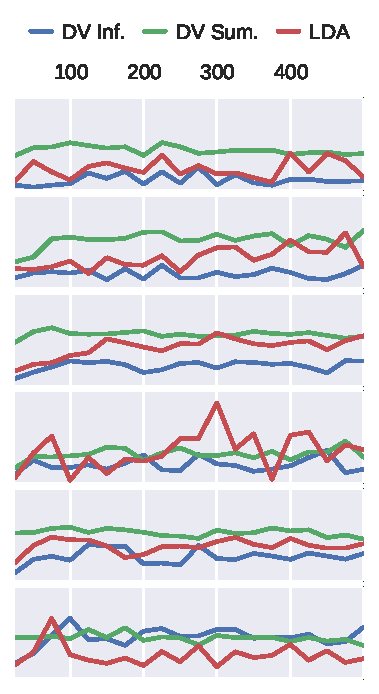
\includegraphics[width=1\textwidth]{../figures/mrr_graph}
        \end{column}
        \end{columns}
        \hfill \hfill

      \end{block}
    \end{minipage}
  \end{beamercolorbox}

  \vskip 1cm

  \end{frame}
\end{document}

